\documentclass[a4paper]{article}
\usepackage{polski}
\usepackage[utf8]{inputenc}
\usepackage{enumerate}
\usepackage{hyperref}
\usepackage{graphicx}

\title{Wizualizacja danych sensorycznych - projekt}
\date{}

\begin{document}
\maketitle

\begin{enumerate}

\item Temat projektu:

Wizualizacja pogody w Japonii.

\item Wykonawca:

Filip Malinowski 209193

\item Opis projektu:

Projektowany program będzie pobierać pogodę z różnych serwisów pogodowych w Japonii. Dane będzie aktualizował dynamicznie co okres czasu wybrany przez użytkownika, np. co 1 minutę, 1 godzinę, 2 godziny. Informacje o pogodzie będą wyświetlane na mapie.

Interaktywność mapy będzie polegać na tym, że domyślnie dla każdej stolicy prefektury będzie wyświetlana temperatura i ikona zachmurzenia. Po kliknięciu na nazwę stolicy prefektury rozwinie się szczegółowa pogoda zawierająca: temperaturę, szansę opadów, ciśnienie, wilgotność,  zachmurzenie, prędkość i kierunek wiatru oraz poziom promieniowania UV. Mapę będzie można również przesuwać oraz zmieniać powiększenie.

W programie będzie również druga zakładka, w której użytkownik będzie mógł wyszukać miasto i wyświetlić dla niego szczegółowe informacje na temat pogody. Wyświetlona zostanie prognoza godzinowa wszystkich czynników podanych wcześniej do wyświetlania na mapie.

Planowane funkcjonalności do wykonania do 22 kwietnia:
\begin{itemize}
\item Wyświetlanie mapy Japonii
\item Poprawne pobieranie informacji o pogodzie dla Tokio
\end{itemize}

Żadnych funkcjonalności aplikacji nie udało się do tej pory zrealizować.

\item Harmonogram:

\begin{description}
\item[9 kwietnia - zrealizowane] | przeprowadzenie badań na temat najlepszych źródeł informacji oraz odpowiedniej struktury programu;

\item[22 kwietnia - niezrealizowane] | napisanie wersji alpha programu realizującej podstawowe funkcje programu. Podstawowymi funkcjami do realizacji są: wyświetlenie mapy Japonii, pobranie danych z serwisów pogodowych i zapisanie ich w klasie danego miasta;

\item[23 kwietnia] | podsumowanie wstępnej wersji programu oraz ewentualne poprawki w planach projektu.
\end{description}

\item Diagram przepływu sterowania:\\
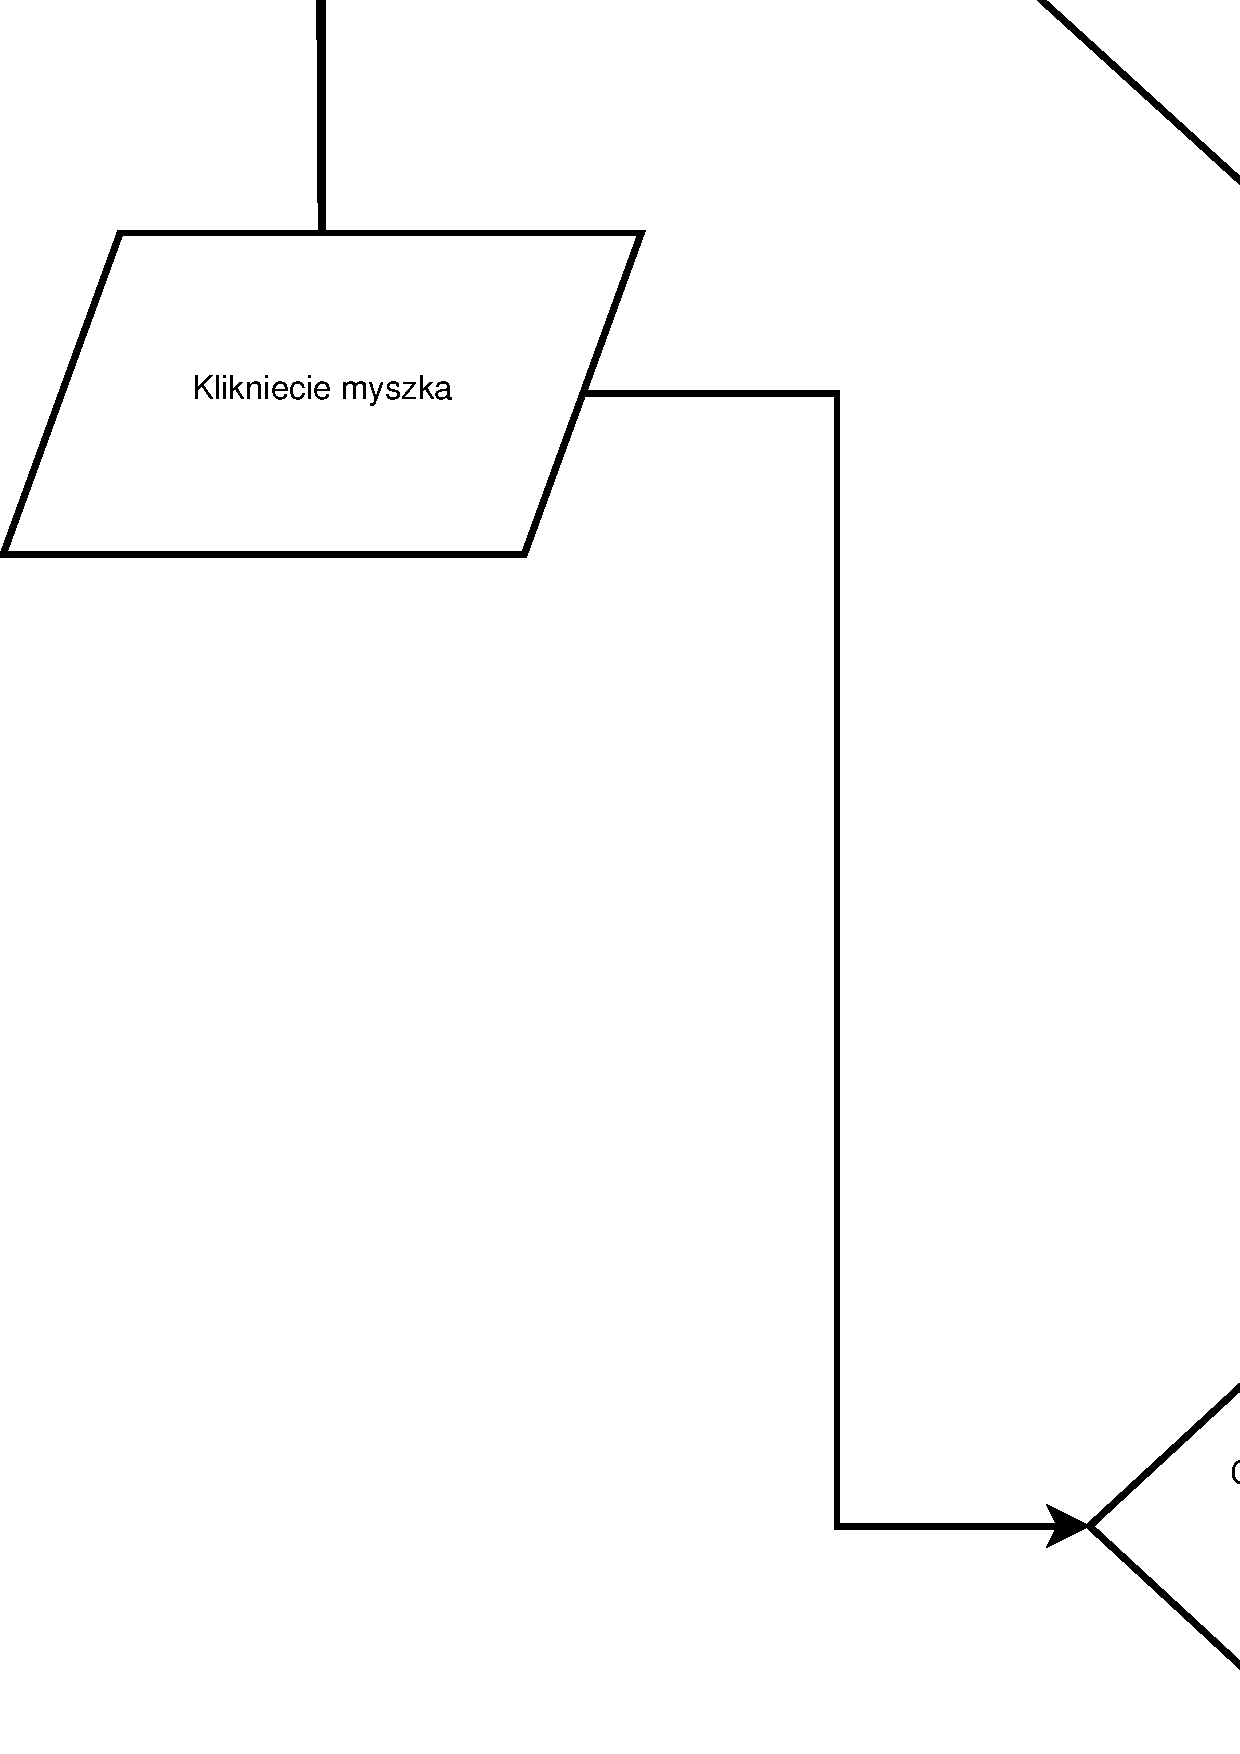
\includegraphics[scale=0.4]{przeplyw.png}

\item Zarządzanie projektem:
\begin{itemize}
\item Git - do przechowywania i rozwijania dokumentacji oraz oprogramowania związanego z projektem.
\href{https://github.com/hizonglol/wds-2016}{Adres internetowy repozytorium.}
\item LaTeX - do tworzenia dokumentacji projektu
\end{itemize}
\end{enumerate}
\end{document}